\documentclass{article}
\usepackage[utf8]{inputenc}
\usepackage{listings}
\usepackage{graphicx}
\usepackage{grffile}
\usepackage{subcaption}
\usepackage[a4paper,top=3cm,bottom=2cm,left=1cm,right=1cm,marginparwidth=1.75cm]{geometry}
\title{TFG informe inicial}
\author{Raquel}
\usepackage[font={footnotesize}]{caption}

\usepackage{natbib}
\usepackage{graphicx}
\usepackage{color}
\definecolor{blue}{RGB}{0,51,102}

\graphicspath{{./pictures/}}

\begin{document}

\maketitle

\tableofcontents

\section{Data}
\subsection{Initial Data}
\begin{itemize}
\item Embedding matrix of size $(50000, 12416)$, con $62080000$ features.
\item \textbf{labels} Labels vector of size $50k$ which every label is in numeric format $(0,999)$
\item \textbf{synsets = synset0 synset1 synset2 ...} The set of synsets that we will analyze: 

$ synsets = [living\_things, mammal, dog, hunting\_dogs]$

\item \textbf{categories = \{-1 0 1 \}} The possible values of the features.
\end{itemize}
\subsection{Generated Data}
\begin{itemize}
\item \textbf{synset\_index\_hyponim.txt} A list with all the hyponims of every synset.


\item \textbf{synset\_index.txt}For each synset a list with the index of the elements of the hyponim list in the embedding.


\item Un diccionario con la cantidad de imágenes que tiene cada feature para cada category. 
\item \textbf{features\_per\_image[synsets].pkl} dfd
\item \textbf{features\_per\_layer[synsets].pkl}dsf
\item \textbf{Images/\_per\_feature\_per\_synset[synsets].pkl} Genera un diccionario tal que:

dict[features][category][synset] = cantidad e imagenes del synset que tienen esta categoria en cuestión.
\item \textbf{intra\_synset[synsets].pkl}fdsfs
\end{itemize}

\section{Objetivos}


\begin{itemize}
\item Estadísticas del dataset por imagen del conjunto de synsets \textbf{(hecho)}
\item Estadísticas internas para cada synset(que synsets son subconjunto de cual y en que proporción)\textbf{(hecho)}
\item Estadísticas totales de la distribución de las features respecto a toda la matriz de imágenes. \textbf{(solo faltan grafiquillas)}
\item  Estadísticas totales de la distribución de las features respecto a toda la matriz de imágenes por layer.\textbf{(falta escribir + grafiquillas)}
\item Estadísticas de las features respecto el subconjunto de imágenes de cada synset. \textbf{(faltan grafiquillas)}
\item Estadísticas de las features respecto el subconjunto de imágenes de cada synset por layer.\textbf{(falta todo)}
\item Distribución de imágenes por feature (para 1, -1, 0):
\begin{itemize}
\item respecto a todas las imágenes
\item respecto a cada uno de los subconjuntos de imágenes de cada synset 
\end{itemize}
\textbf{está calculado, falta escribir}
\item Repetir para el resto de embeddings
\item Montarlo para que me genere todo automático para cada conjunto de synsets.
\item Hacer que guarde todo en maps  
\item Features por imagen: Para cada imagen cuantas features (de cada category) se activan. Usando todos los valores obtenidos dibujo un histograma
para cada category de feature. Con el eje de las x siendo la frecuencia y el de las y la cantidad de imágenes que cumplen eso.
\item Imágenes por feature: Para cada features (de cada category), cuantas imágenes toman este valor. Usando todos los valores obtenidos dibujo un histograma
para cada category de feature. Con el eje de las x siendo la frecuencia y el de las y la cantidad de imágenes que cumplen eso.  
\item Comprobar si dentro de un mismo synset hay features que se den con 1 y -1.
\item Hacer las distribuciones de la suma.
\item Ordenar del código y generar una documentación y tests.

\end{itemize}

\newpage

\section{Análisis Base}

\begin{figure}[h] 
	\centering 
	\includegraphics[width=0.45\textwidth] {['living_thing', 'mammal', 'dog', 'hunting_dog']19/plots/distribution_of_synsets_bar.png}  
	\includegraphics[width=0.45\textwidth]{['artifact', 'instrumentality', 'conveyance', 'wheeled_vehicle']19/plots/distribution_of_synsets_bar.png}
\end{figure}
 
%\begin{figure}
%\centering
%\begin{subfigure}[b]{0.4\textwidth}
%\includegraphics[width=\textwidth] {['living_thing', 'mammal', 'dog', 'hunting_dog']19/plots/distribution_of_synsets_bar.png}  
%  \end{subfigure}
% \begin{subfigure}[b]{0.4\textwidth}
%\includegraphics[width=\textwidth]{['artifact', 'instrumentality', 'conveyance', 'wheeled_vehicle']19/plots/distribution_of_synsets_bar.png}
%  \end{subfigure}
% \end{figure}

\subsection{Intra sinset}

%\texttt{%\begin{figure}[h] 
% \centering 
% \includegraphics[scale=0.3] {['living_thing', 'mammal', 'dog', 'hunting_dog']19/plots/distribution_of_inter_synsets_bar_living_thing.png} 
%\includegraphics[scale=0.3] {['living_thing', 'mammal', 'dog', 'hunting_dog']25/plots/distribution_of_inter_synsets_bar_living_thing.png} 
%\includegraphics[scale=0.3] {['living_thing', 'mammal', 'dog', 'hunting_dog']31/plots/distribution_of_inter_synsets_bar_living_thing.png} 
% \end{figure}
%\begin{figure}[h] 
% \centering 
% 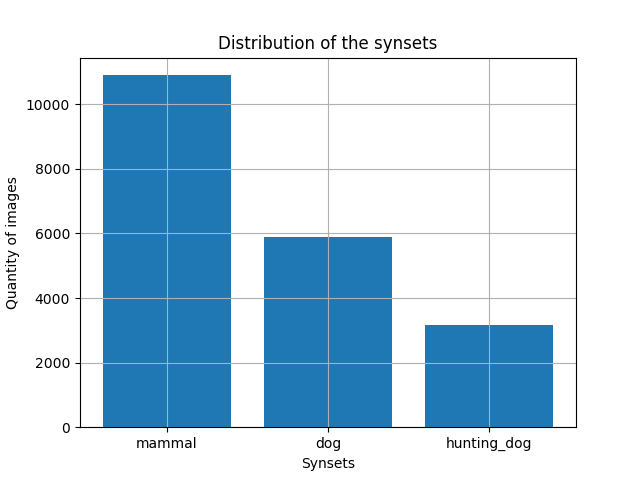
\includegraphics[scale=0.3] {['living_thing', 'mammal', 'dog', 'hunting_dog']19/plots/distribution_of_inter_synsets_bar_mammal.png} 
% \end{figure}
%\begin{figure}[h] 
% \centering 
% 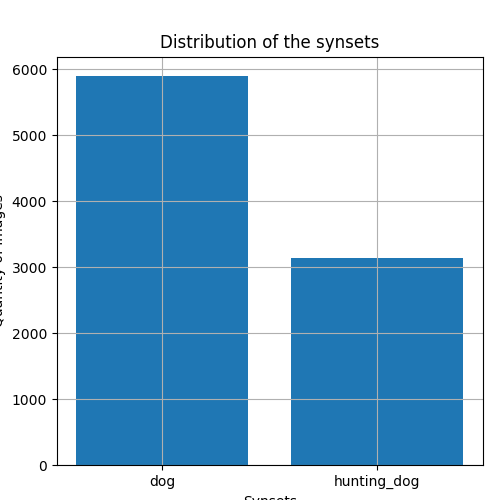
\includegraphics[width=0.45\textwidth] {['living_thing', 'mammal', 'dog', 'hunting_dog']19/plots/distribution_of_inter_synsets_bar_dog.png} 
% \end{figure}}
\begin{figure}[h] 
	\centering 
	\begin{subfigure}[b]{0.45\textwidth}
		\includegraphics[width=\textwidth] {['living_thing', 'mammal', 'dog', 'hunting_dog']19/plots/distribution_of_synsets_bar.png} 
		\caption*{Living Things} 
	\end{subfigure}
	\begin{subfigure}[b]{0.45\textwidth}
	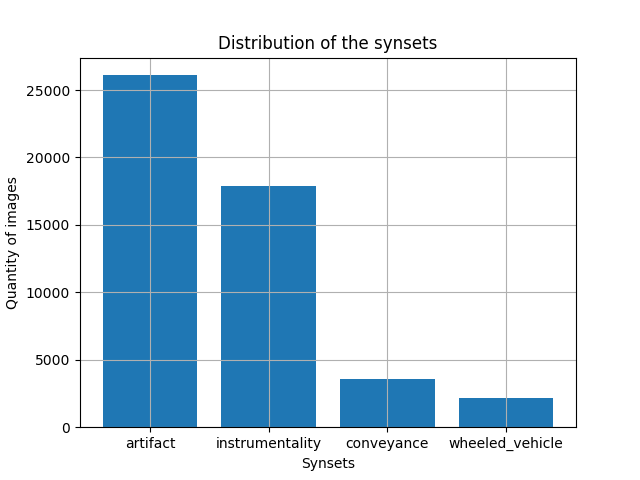
\includegraphics[width=\textwidth]{['artifact', 'instrumentality', 'conveyance', 'wheeled_vehicle']19/plots/distribution_of_inter_synsets_bar_artifact.png}
	\caption*{Non Living Things} 
	\end{subfigure}
\end{figure}

\begin{figure}[h] 
	\centering 
	\includegraphics[width=0.45\textwidth] {['living_thing', 'mammal', 'dog', 'hunting_dog']19/plots/distribution_of_inter_synsets_bar_living_thing.png}  
	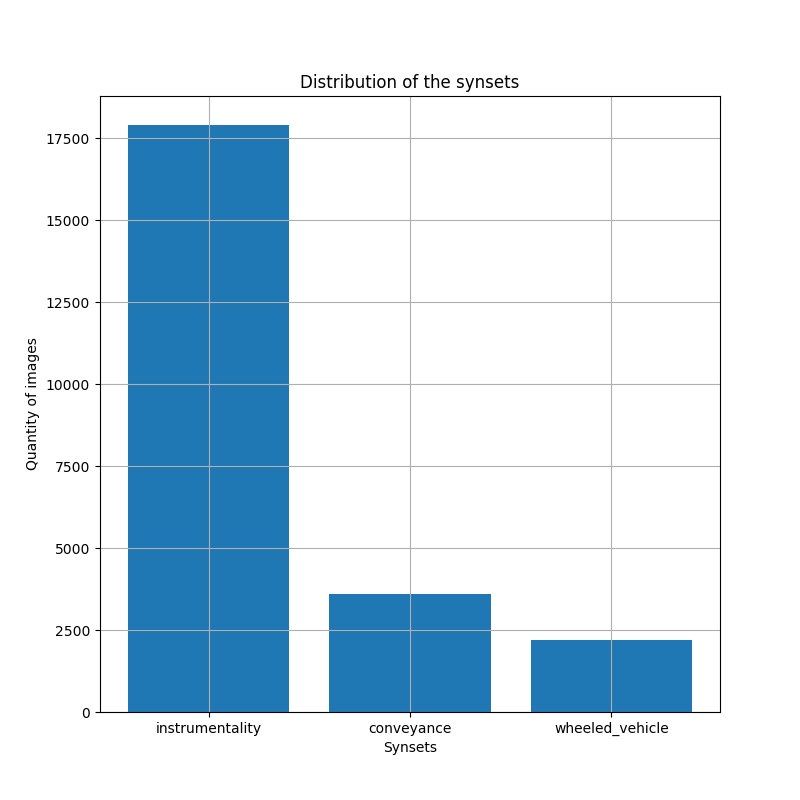
\includegraphics[width=0.45\textwidth]{['artifact', 'instrumentality', 'conveyance', 'wheeled_vehicle']19/plots/distribution_of_inter_synsets_bar_instrumentality.png}
\end{figure}

\begin{figure}[h] 
	\centering 
	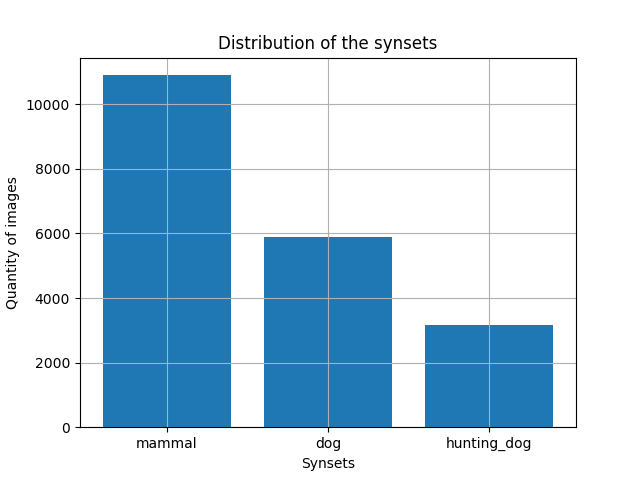
\includegraphics[width=0.45\textwidth] {['living_thing', 'mammal', 'dog', 'hunting_dog']19/plots/distribution_of_inter_synsets_bar_mammal.png}  
	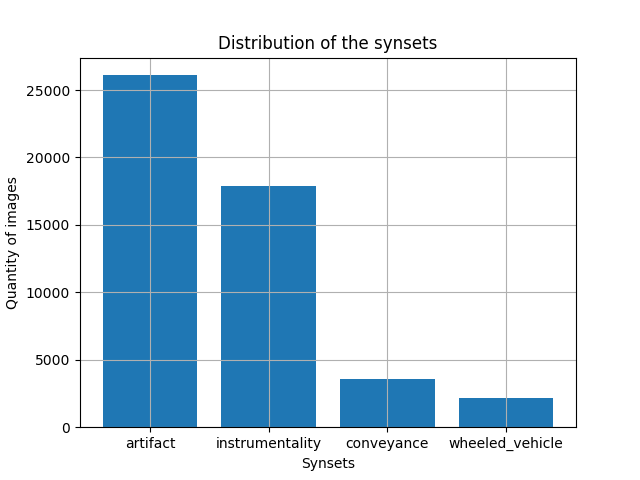
\includegraphics[width=0.45\textwidth]{['artifact', 'instrumentality', 'conveyance', 'wheeled_vehicle']19/plots/distribution_of_inter_synsets_bar_artifact.png}
\end{figure}

\begin{figure}[h] 
	\centering 
	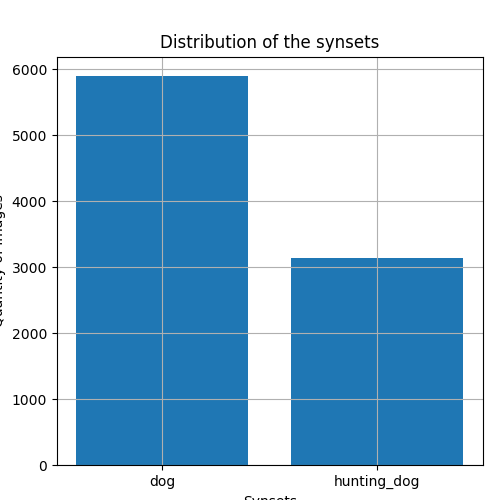
\includegraphics[width=0.45\textwidth] {['living_thing', 'mammal', 'dog', 'hunting_dog']19/plots/distribution_of_inter_synsets_bar_dog.png}  
	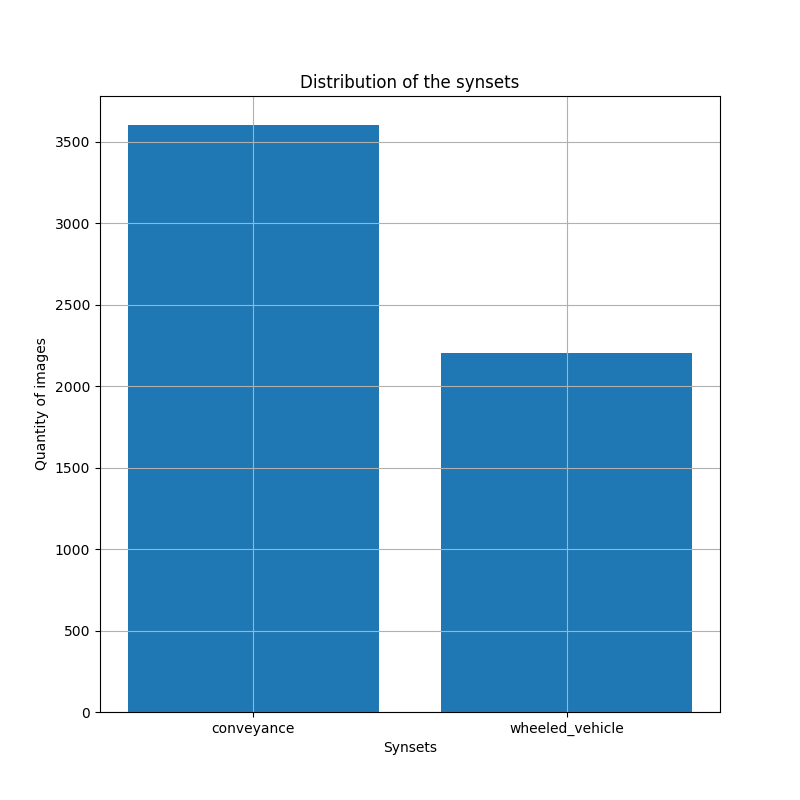
\includegraphics[width=0.45\textwidth]{['artifact', 'instrumentality', 'conveyance', 'wheeled_vehicle']19/plots/distribution_of_inter_synsets_bar_conveyance.png}
\end{figure}

\begin{figure}[h] 
	\centering 
	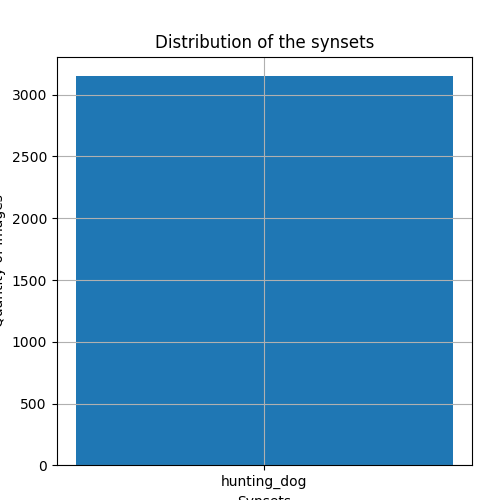
\includegraphics[width=0.45\textwidth] {['living_thing', 'mammal', 'dog', 'hunting_dog']19/plots/distribution_of_inter_synsets_bar_hunting_dog.png}  
	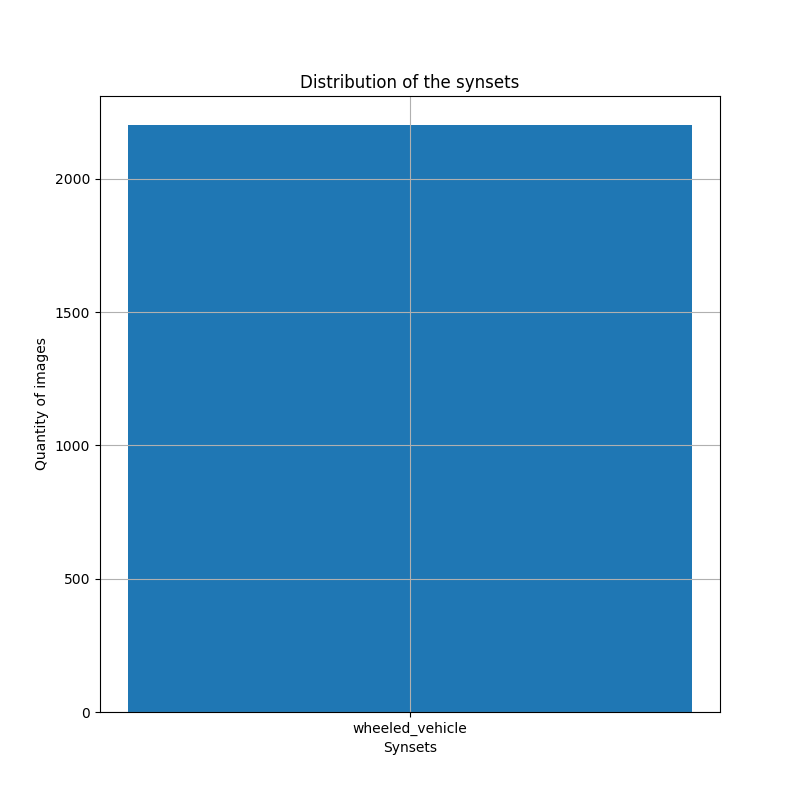
\includegraphics[width=0.45\textwidth]{['artifact', 'instrumentality', 'conveyance', 'wheeled_vehicle']19/plots/distribution_of_inter_synsets_bar_wheeled_vehicle.png}
\end{figure}

 \newpage
 \clearpage
\subsection{Distribución total de las features}

%\begin{figure}[h] 
%	\centering 
%	\begin{subfigure}[b]{0.45\textwidth}
%		  \includegraphics[width=\textwidth] {['living_thing', 'mammal', 'dog', 'hunting_dog']19/plots/quantity_of_features_bar.png} 
%		\caption*{Living Things} 
%	\end{subfigure}
%	\begin{subfigure}[b]{0.45\textwidth}
%	 \includegraphics[width=\textwidth] {['artifact', 'instrumentality', 'conveyance', 'wheeled_vehicle']19/plots/quantity_of_features_bar.png} 
%	\caption*{Non Living Things} 
%	\end{subfigure}
%	\caption*{Embedding 19}
%\end{figure}
%
%\begin{figure}[h] 
%	\centering 
%	\begin{subfigure}[b]{0.45\textwidth}
%		 \includegraphics[width=\textwidth] {['living_thing', 'mammal', 'dog', 'hunting_dog']25/plots/quantity_of_features_bar.png} 
%		\caption*{Living Things} 
%	\end{subfigure}
%	\begin{subfigure}[b]{0.45\textwidth}
%	 \includegraphics[width=\textwidth] {['artifact', 'instrumentality', 'conveyance', 'wheeled_vehicle']25/plots/quantity_of_features_bar.png} 
%	\caption*{Non Living Things} 
%	\end{subfigure}
%	\caption*{Embedding 25}
%\end{figure}
%
%\begin{figure}[h] 
%	\centering 
%	\begin{subfigure}[b]{0.45\textwidth}
%		 \includegraphics[width=\textwidth] {['living_thing', 'mammal', 'dog', 'hunting_dog']31/plots/quantity_of_features_bar.png} 
%		\caption*{Living Things} 
%	\end{subfigure}
%	\begin{subfigure}[b]{0.45\textwidth}
%	 \includegraphics[width=\textwidth] {['artifact', 'instrumentality', 'conveyance', 'wheeled_vehicle']31/plots/quantity_of_features_bar.png} 
%	\caption*{Non Living Things} 
%	\end{subfigure}
%	\caption*{Embedding 31}
%\end{figure}

\begin{figure}[h] 
 \centering 
	\begin{subfigure}[b]{0.3\textwidth}
 		\includegraphics[width=\textwidth] {['living_thing', 'mammal', 'dog', 'hunting_dog']19/plots/quantity_of_features_bar.png}
 		\caption*{Embedding 19}
 	\end{subfigure}
 	\begin{subfigure}[b]{0.3\textwidth}
 		\includegraphics[width=\textwidth] {['living_thing', 'mammal', 'dog', 'hunting_dog']25/plots/quantity_of_features_bar.png}
 		\caption*{Embedding 25}
 	\end{subfigure}
 	\begin{subfigure}[b]{0.3\textwidth}
 		\includegraphics[width=\textwidth] {['living_thing', 'mammal', 'dog', 'hunting_dog']31/plots/quantity_of_features_bar.png}
 		\caption*{Embedding 31}
 	\end{subfigure}
 \end{figure}

 
 \begin{figure}[h] 
 \centering 
 \end{figure}
 
\subsection{Distribución de las features por layer}

\begin{figure}[h] 
 \centering 
	\begin{subfigure}[b]{0.3\textwidth}
 		\includegraphics[width=\textwidth] {['living_thing', 'mammal', 'dog', 'hunting_dog']19/plots/features_per_layer_of_conv1.png}
 		\caption*{Embedding 19}
 	\end{subfigure}
 	\begin{subfigure}[b]{0.3\textwidth}
 		\includegraphics[width=\textwidth] {['living_thing', 'mammal', 'dog', 'hunting_dog']25/plots/features_per_layer_of_conv1.png}
 		\caption*{Embedding 25}
 	\end{subfigure}
 	\begin{subfigure}[b]{0.3\textwidth}
 		\includegraphics[width=\textwidth] {['living_thing', 'mammal', 'dog', 'hunting_dog']31/plots/features_per_layer_of_conv1.png}
 		\caption*{Embedding 31}
 	\end{subfigure}
 \end{figure}
 
 

 \begin{figure}[h] 
            \centering
            \begin{subfigure}[b]{0.3\textwith}
            \includegraphics[width=\textwith] {['living_thing', 'mammal', 'dog', 'hunting_dog']19/plots/features_per_layer_of_conv2.png}
            \caption*{Embedding 19}
 	        \end{subfigure}
            \begin{subfigure}[b]{0.3\textwith}
            \includegraphics[width=\textwith] {['living_thing', 'mammal', 'dog', 'hunting_dog']25/plots/features_per_layer_of_conv2.png}
            \caption*{Embedding 25}
 	        \end{subfigure}
            \begin{subfigure}[b]{0.3\textwith}
            \includegraphics[width=\textwith] {['living_thing', 'mammal', 'dog', 'hunting_dog']31/plots/features_per_layer_of_conv2.png}
            \caption*{Embedding 31}
 	        \end{subfigure}       
        \end{figure}
        
       \begin{figure}[h] 
            \centering
            \begin{subfigure}[b]{0.3\textwith}
            \includegraphics[width=\textwith] {['living_thing', 'mammal', 'dog', 'hunting_dog']19/plots/features_per_layer_of_conv3.png}
            \caption*{Embedding 19}
 	        \end{subfigure}
            \begin{subfigure}[b]{0.3\textwith}
            \includegraphics[width=\textwith] {['living_thing', 'mammal', 'dog', 'hunting_dog']25/plots/features_per_layer_of_conv3.png}
            \caption*{Embedding 25}
 	        \end{subfigure}
            \begin{subfigure}[b]{0.3\textwith}
            \includegraphics[width=\textwith] {['living_thing', 'mammal', 'dog', 'hunting_dog']31/plots/features_per_layer_of_conv3.png}
            \caption*{Embedding 31}
 	        \end{subfigure}       
        \end{figure}
        
       \begin{figure}[h] 
            \centering
            \begin{subfigure}[b]{0.3\textwith}
            \includegraphics[width=\textwith] {['living_thing', 'mammal', 'dog', 'hunting_dog']19/plots/features_per_layer_of_conv4.png}
            \caption*{Embedding 19}
 	        \end{subfigure}
            \begin{subfigure}[b]{0.3\textwith}
            \includegraphics[width=\textwith] {['living_thing', 'mammal', 'dog', 'hunting_dog']25/plots/features_per_layer_of_conv4.png}
            \caption*{Embedding 25}
 	        \end{subfigure}
            \begin{subfigure}[b]{0.3\textwith}
            \includegraphics[width=\textwith] {['living_thing', 'mammal', 'dog', 'hunting_dog']31/plots/features_per_layer_of_conv4.png}
            \caption*{Embedding 31}
 	        \end{subfigure}       
        \end{figure}
        
       \begin{figure}[h] 
            \centering
            \begin{subfigure}[b]{0.3\textwith}
            \includegraphics[width=\textwith] {['living_thing', 'mammal', 'dog', 'hunting_dog']19/plots/features_per_layer_of_conv5.png}
            \caption*{Embedding 19}
 	        \end{subfigure}
            \begin{subfigure}[b]{0.3\textwith}
            \includegraphics[width=\textwith] {['living_thing', 'mammal', 'dog', 'hunting_dog']25/plots/features_per_layer_of_conv5.png}
            \caption*{Embedding 25}
 	        \end{subfigure}
            \begin{subfigure}[b]{0.3\textwith}
            \includegraphics[width=\textwith] {['living_thing', 'mammal', 'dog', 'hunting_dog']31/plots/features_per_layer_of_conv5.png}
            \caption*{Embedding 31}
 	        \end{subfigure}       
        \end{figure}
        
        
         \begin{figure}[h] 
            \centering
            \begin{subfigure}[b]{0.3\textwith}
            \includegraphics[width=\textwith] {['living_thing', 'mammal', 'dog', 'hunting_dog']19/plots/features_per_layer_of_fc6.png}
            \caption*{Embedding 19}
 	        \end{subfigure}
            \begin{subfigure}[b]{0.3\textwith}
            \includegraphics[width=	extwidth] {['living_thing', 'mammal', 'dog', 'hunting_dog']25/plots/features_per_layer_of_fc6.png}
            \caption*{Embedding 25}
 	        \end{subfigure}
            \begin{subfigure}[b]{0.3\textwith}
            \includegraphics[width=\textwith] {['living_thing', 'mammal', 'dog', 'hunting_dog']31/plots/features_per_layer_of_fc6.png}
            \caption*{Embedding 31}
 	        \end{subfigure}       
        \end{figure}
        
       \begin{figure}[h] 
            \centering
            \begin{subfigure}[b]{0.3\textwith}
            \includegraphics[width=\textwith] {['living_thing', 'mammal', 'dog', 'hunting_dog']19/plots/features_per_layer_of_fc7.png}
            \caption*{Embedding 19}
 	        \end{subfigure}
            \begin{subfigure}[b]{0.3\textwith}
            \includegraphics[width=\textwith] {['living_thing', 'mammal', 'dog', 'hunting_dog']25/plots/features_per_layer_of_fc7.png}
            \caption*{Embedding 25}
 	        \end{subfigure}
            \begin{subfigure}[b]{0.3\textwith}
            \includegraphics[width=\textwith] {['living_thing', 'mammal', 'dog', 'hunting_dog']31/plots/features_per_layer_of_fc7.png}
            \caption*{Embedding 31}
 	        \end{subfigure}       
        \end{figure}
\newpage
\clearpage

\subsection{Distribución de las features por synset}

\begin{figure}[h] 
 \centering 
 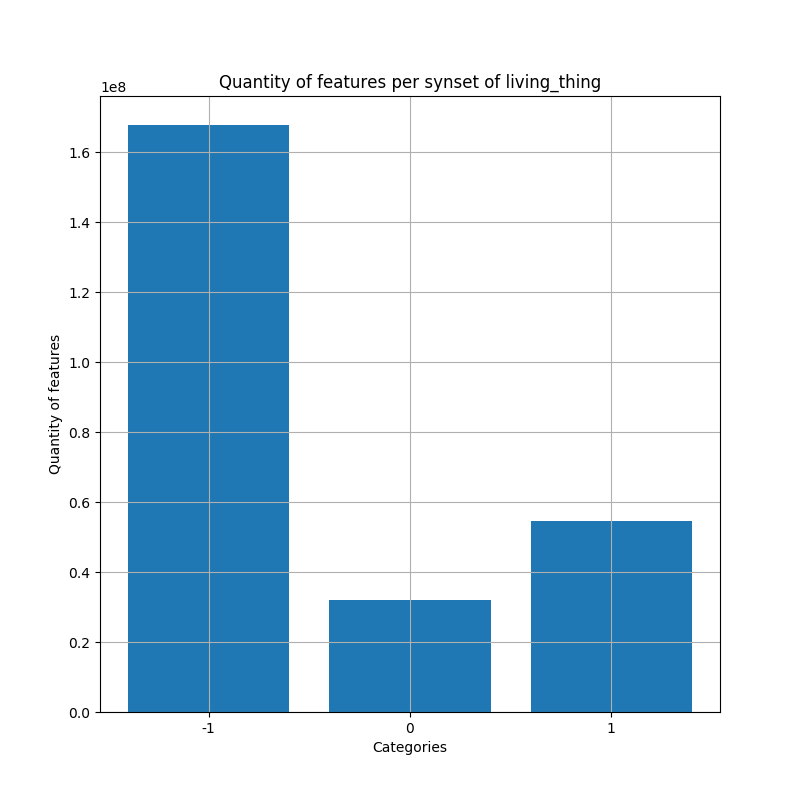
\includegraphics[width=0.45\textwidth] {['living_thing', 'mammal', 'dog', 'hunting_dog']19/plots/features_per_synset_bar_living_thing.png} 
 \end{figure}

\begin{figure}[h] 
 \centering 
 \includegraphics[width=0.45\textwidth] {['living_thing', 'mammal', 'dog', 'hunting_dog']19/plots/features_per_synset_bar_mammal.png} 
 \end{figure}


\begin{figure}[h] 
 \centering 
 \includegraphics[width=0.45\textwidth] {['living_thing', 'mammal', 'dog', 'hunting_dog']19/plots/features_per_synset_bar_dog.png} 
 \end{figure}


\begin{figure}[h] 
 \centering 
 \includegraphics[width=0.45\textwidth] {['living_thing', 'mammal', 'dog', 'hunting_dog']19/plots/features_per_synset_bar_hunting_dog.png} 
 \end{figure}



\newpage
\clearpage
\subsection{Features per image}
%Calculo para cada imagen las features que se activan, respecto la matriz total de datos.
There are for each image the total counting of features active, for the different possible categories ($-1,0,1$):
\begin{figure}[h] 
 \centering 
 \includegraphics[width=0.45\textwidth] {['living_thing', 'mammal', 'dog', 'hunting_dog']19/plots/features_per_image-1} 
 \end{figure}
\begin{figure}[h] 
 \centering 
 \includegraphics[width=0.45\textwidth] {['living_thing', 'mammal', 'dog', 'hunting_dog']19/plots/features_per_image0} 
 \end{figure}
\begin{figure}[h] 
 \centering 
 \includegraphics[width=0.45\textwidth] {['living_thing', 'mammal', 'dog', 'hunting_dog']19/plots/features_per_image1} 
 \end{figure}


\newpage
\clearpage
\subsection{Images per feature}
Now I calculate for each feature how many images activate in each specific category:
\begin{figure}[h] 
 \centering 
 \includegraphics[width=0.45\textwidth] {['living_thing', 'mammal', 'dog', 'hunting_dog']19/plots/Images_per_feature_of_-1_category.png} 
 \end{figure}
\begin{figure}[h] 
 \centering 
 \includegraphics[width=0.45\textwidth] {['living_thing', 'mammal', 'dog', 'hunting_dog']19/plots/Images_per_feature_of_-1_category_box.png} 
 \end{figure}
\begin{figure}[h] 
 \centering 
 \includegraphics[width=0.45\textwidth] {['living_thing', 'mammal', 'dog', 'hunting_dog']19/plots/Images_per_feature_of_0_category.png} 
 \end{figure}
\begin{figure}[h] 
 \centering 
 \includegraphics[width=0.45\textwidth] {['living_thing', 'mammal', 'dog', 'hunting_dog']19/plots/Images_per_feature_of_0_category_box.png} 
 \end{figure}
\begin{figure}[h] 
 \centering 
 \includegraphics[width=0.45\textwidth] {['living_thing', 'mammal', 'dog', 'hunting_dog']19/plots/Images_per_feature_of_1_category.png} 
 \end{figure}
\begin{figure}[h] 
 \centering 
 \includegraphics[width=0.45\textwidth] {['living_thing', 'mammal', 'dog', 'hunting_dog']19/plots/Images_per_feature_of_1_category_box.png} 
 \end{figure}

\newpage
\clearpage


\subsection{Images per feature per synset}

\begin{figure}[h] 
 \centering 
 \includegraphics[width=0.45\textwidth] {['living_thing', 'mammal', 'dog', 'hunting_dog']19/plots/Images_per_feature_of_-1_category_living_thing.png} 
 \end{figure}
\begin{figure}[h] 
 \centering 
 \includegraphics[width=0.45\textwidth] {['living_thing', 'mammal', 'dog', 'hunting_dog']19/plots/Images_per_feature_of_0_category_living_thing.png} 
 \end{figure}
\begin{figure}[h] 
 \centering 
 \includegraphics[width=0.45\textwidth] {['living_thing', 'mammal', 'dog', 'hunting_dog']19/plots/Images_per_feature_of_1_category_living_thing.png} 
 \end{figure}
\begin{figure}[h] 
 \centering 
 \includegraphics[width=0.45\textwidth] {['living_thing', 'mammal', 'dog', 'hunting_dog']19/plots/Images_per_feature_of_-1_category_mammal.png} 
 \end{figure}
\begin{figure}[h] 
 \centering 
 \includegraphics[width=0.45\textwidth] {['living_thing', 'mammal', 'dog', 'hunting_dog']19/plots/Images_per_feature_of_0_category_mammal.png} 
 \end{figure}
\begin{figure}[h] 
 \centering 
 \includegraphics[width=0.45\textwidth] {['living_thing', 'mammal', 'dog', 'hunting_dog']19/plots/Images_per_feature_of_1_category_mammal.png} 
 \end{figure}
\begin{figure}[h] 
 \centering 
 \includegraphics[width=0.45\textwidth] {['living_thing', 'mammal', 'dog', 'hunting_dog']19/plots/Images_per_feature_of_-1_category_dog.png} 
 \end{figure}
\begin{figure}[h] 
 \centering 
 \includegraphics[width=0.45\textwidth] {['living_thing', 'mammal', 'dog', 'hunting_dog']19/plots/Images_per_feature_of_0_category_dog.png} 
 \end{figure}
\begin{figure}[h] 
 \centering 
 \includegraphics[width=0.45\textwidth] {['living_thing', 'mammal', 'dog', 'hunting_dog']19/plots/Images_per_feature_of_1_category_dog.png} 
 \end{figure}
\begin{figure}[h] 
 \centering 
 \includegraphics[width=0.45\textwidth] {['living_thing', 'mammal', 'dog', 'hunting_dog']19/plots/Images_per_feature_of_-1_category_hunting_dog.png} 
 \end{figure}
\begin{figure}[h] 
 \centering 
 \includegraphics[width=0.45\textwidth] {['living_thing', 'mammal', 'dog', 'hunting_dog']19/plots/Images_per_feature_of_0_category_hunting_dog.png} 
 \end{figure}
\begin{figure}[h] 
 \centering 
 \includegraphics[width=0.45\textwidth] {['living_thing', 'mammal', 'dog', 'hunting_dog']19/plots/Images_per_feature_of_1_category_hunting_dog.png} 
 \end{figure}



\newpage
\clearpage


\subsection{Comprobación de que las cosas tinen sentido}
\begin{itemize}
\item \textbf{Hay alguna imagen que no tenga ninguna feature con valor cero? } No, ninguna
\item \textbf{Hay algun synset que tenga valor 1 y -1 para la misma feature? } Si, bastantes.
Estamos tomando: 

La feature tiene el valor i para el synset si lo tiene para alguna imagen del synset(Estamos estudiando la submatriz correspondiente al synset)
\end{itemize}
\subsection{Estudio de los outliers de imagenes per feature}


\begin{figure}[h] 
 \centering 
 \includegraphics[width=0.45\textwidth] {['living_thing', 'mammal', 'dog', 'hunting_dog']19/plots/outliers-1.png} 
 \caption{ Category: -1}
 \end{figure}
\begin{figure}[h] 
 \centering 
 \includegraphics[width=0.45\textwidth] {['living_thing', 'mammal', 'dog', 'hunting_dog']19/plots/outliers0.png} 
 \caption{ Category: 0}
 \end{figure}
\begin{figure}[h] 
 \centering 
 \includegraphics[width=0.45\textwidth] {['living_thing', 'mammal', 'dog', 'hunting_dog']19/plots/outliers1.png} 
  \caption{ Category: 1}
 \end{figure}




\end{document}
\grid
